\documentclass{homework}

\title{Homework 3}
\begin{document}
    \maketitle

    \problem
    \begin{proof}
        Denote $X_t:=W_t^2$, then by Doob's submartingale inequality
        we have that
        \[P\left(\max_{0\leq s\leq t}X_s\geq\lambda\right)
        \leq\frac{1}{\lambda}E(X_t^+)=\frac{t}{\lambda}\]
        as $X_t\geq 0$ implies $E(X_t^+)=E(X_t)=t$. Hence the
        first inequality is proved.

        Since
        \[\begin{aligned}
            E(|W_t|)&=\int_{\Omega}W_t\diff P\\
            &=\int_{-\infty}^\infty x\cdot
              \frac{\e^{-\frac{x^2}{2t}}}{\sqrt{2\pi t}}
              \diff x\\
            &=\sqrt{\frac{2}{\pi t}}\int_0^\infty x\e^{-\frac{x^2}{2t}}\diff x\\
            &=\sqrt{\frac{2}{\pi t}}\int_0^\infty \e^{-\frac{\xi}{t}}\diff\xi\\
            &=\sqrt{\frac{2t}{\pi}}
        \end{aligned}\]
        where we use $\xi=x^2/2$ as a substitution,
        then we know that
        \[E(|W_t|^+)=E(|W_t|)=\sqrt{\frac{2t}{\pi}}\]
        hence by Doob's inequality we obtain
        \[P\left(\max_{0\leq s\leq t}|W_t|\geq\lambda\right)
        \leq\frac{1}{\lambda}E(|W_t|^+)=\frac{\sqrt{2t/\pi}}{\lambda}\]
        which is the statement of the second inequality
        \sidenote{It seems like that you typed $\frac{\sqrt{2t/\pi}}{\lambda}$
        as $\frac{\sqrt{2t/\lambda}}{\lambda}$ by mistake.}.
    \end{proof}

    \problem
    \begin{proof}
        To prove convergence in probability, consider
        $\forall\sigma>0$,
        \[P(|X_t|\geq\sigma)
        =P\left(\max_{0\leq s\leq t}|W_s|\geq\sigma t\right)\]
        then applying Doob's submartingale inequality we have that
        \[P(|X_t|\geq\sigma)\leq\frac{1}{\sigma t}E(|W_s|^+)\]

        Note that existence of $E(W_t)$ yields that
        $E(|W_s|^+)=E(|W_s|)<\infty$, it follows that
        \[P(|X_t|\geq\sigma)\to 0\quad (t\to +\infty)\]
        for a given $\sigma$, hence $X_t\to 0$ in probability
        as $t\to +\infty$.
    \end{proof}

    \problem
    For any random variable $X$ and $p>0$, denote stochastic process
    $Y_t=|X|^p,t\geq 0$,
    then it is obvious that
    \[\max_{0\leq s\leq t}Y_s=|X|^p\]
    Doob's submartingale inequality tells us that
    for any $\lambda>0$
    \[P\left(\max_{0\leq s\leq t}Y_s\geq\lambda^p\right)
    \leq\frac{1}{\lambda^p}E(Y_t^+)\]

    Since $Y_t=|X|^p\geq 0$, we have that
    \[E(Y_t^+)=E(Y_t)=E(|X|^p)\]
    hence
    \[P(|X|^p\geq\lambda^p)\leq\frac{1}{\lambda^p}E(|X|^p)\]
    Also note that
    \[\{\omega\in\Omega;|X(\omega)|^p\geq\lambda^p\}
    =\{\omega\in\Omega;|X(\omega)|\geq\lambda\}\]
    It follows that
    \[P(|X|\geq\lambda)\leq\frac{1}{\lambda^p}E(|X|^p)\]
    which is the statement of Markov inequality.

    \problem
    \newcommand{\absdelta}{\left|X\left(\frac{i+1}{2^n}\right)-X\left(\frac{i}{2^n}\right)\right|}
    \begin{subproblem}
        \item
        \begin{proof}
            Since for any $\omega\in A_n$, there exists some
            integer\sidenote{It seems like there are some mistakes in your
            definition, and I guess
            \begin{multline*}
                A_n:=
                \left\{\absdelta\right.\\
                \left.>\frac{1}{2^{\gamma n}}
                \text{ for some integer }0\leq i\leq 2^n\right\}
            \end{multline*} is what you really mean to.}
            $0\leq i\leq 2^n$, s.t.
            \begin{equation}
                \label{eq:absdelta condi}
                \absdelta>\frac{1}{2^{\gamma n}}
            \end{equation}
            And denote
            \[M_{ni}:=\left\{\absdelta>\frac{1}{2^{\gamma n}}\right\}\]
            then
            \[\omega\in\bigcup_{i=0}^{2^n}M_{ni}\]
            and conversely for any $\omega$ satisfies the condition above,
            $\omega$ satisfies \cref{eq:absdelta condi} too, thus,
            \[A_n=\bigcup_{i=0}^{2^n}M_{ni}\]

            Consider that
            \[\begin{aligned}
                E\left(\absdelta^\beta\right)&=\int_\Omega\absdelta^\beta\diff P\\
                &\geq\int_{M_{ni}}\absdelta^\beta\diff P\\
                &>\int_{M_{ni}}\left(\frac{1}{2^{\gamma n}}\right)^\beta\diff P\\
                &=\frac{P(M_{ni})}{2^{\beta\gamma n}}
            \end{aligned}\]
            And since there exists constant $C,\alpha,\beta$ s.t.
            \[E\left(\absdelta^\beta\right)
            \leq C\left|\frac{i+1}{2^n}-\frac{i}{2^n}\right|^{1+\alpha}
            =\frac{C}{2^{n(1+\alpha)}}\]
            then we have that
            \[\frac{P(M_{ni})}{2^{n\beta\gamma}}
            <\frac{C}{2^{n(1+\alpha)}}\]
            i.e.,
            \[P(M_{ni})<C\cdot 2^{-n(1+\alpha-\beta\gamma)}\]
            It follows that
            \[\begin{aligned}
                P(A_n)&\leq\sum_{i=1}^{2^n}P(M_{ni})\\
                &<\sum_{i=1}^{2^n}C\cdot 2^{-n(1+\alpha-\beta\gamma)}\\
                &=2^n\cdot 2^{-n(1+\alpha-\beta\gamma)}C\\
                &=C\cdot 2^{-(\alpha-\beta\gamma)n}
            \end{aligned}\]
        \end{proof}

        \item
        \begin{proof}
            Since $\gamma<\alpha/\beta$, then $\alpha-\beta\gamma>0$.
            It follows that
            \[\sum_{n=1}^\infty C\cdot 2^{-(\alpha-\beta\gamma)n}\]
            is convergent. Hence,
            \[\sum_{n=1}^\infty P(A_n)
            \leq\sum_{n=1}^\infty C\cdot 2^{-(\alpha-\beta\gamma)n}
            <\infty\]
            then by Borel-Cantelli Lemma, we have that
            \[P\left(\limsup_{n\to\infty}A_n\right)=0\]
            which is equivalent to
            \[P\left(\liminf_{n\to\infty}A_n^\mathrm c\right)=1\]
            where $A_n^\mathrm c$ represents the complement of $A_n$.
            Then by the definition,
            \[\liminf_{n\to\infty}A_n^\mathrm c
            =\bigcup_{N=1}^\infty\bigcap_{n=N}^\infty
            \left\{\absdelta\leq\frac{1}{2^{\gamma n}}\right\}\]
            That being said, for a.e. $\omega\in\Omega$, the following
            holds for any $n$ sufficiently large
            \[\absdelta\leq\frac{1}{2^{\gamma n}}\]
        \end{proof}
    \end{subproblem}

    \problem
    As we can see (\cref{fig:simulation}), the bigger $\sigma$ means more
    powerful zigzag, and $\mu$ determines the main trend,
    while larger $T$ shows something interesting, that though
    a path with higher $\sigma$ goes below one with lower
    during a short time $\sigma$ ($T=5$),
    it overtakes another in the long time ($T=10$).

    Basically $\mu$ is the main stream of motion while
    $\sigma$ is the magnitude of the uncertainity.

    \begin{figure*}
        \centering
        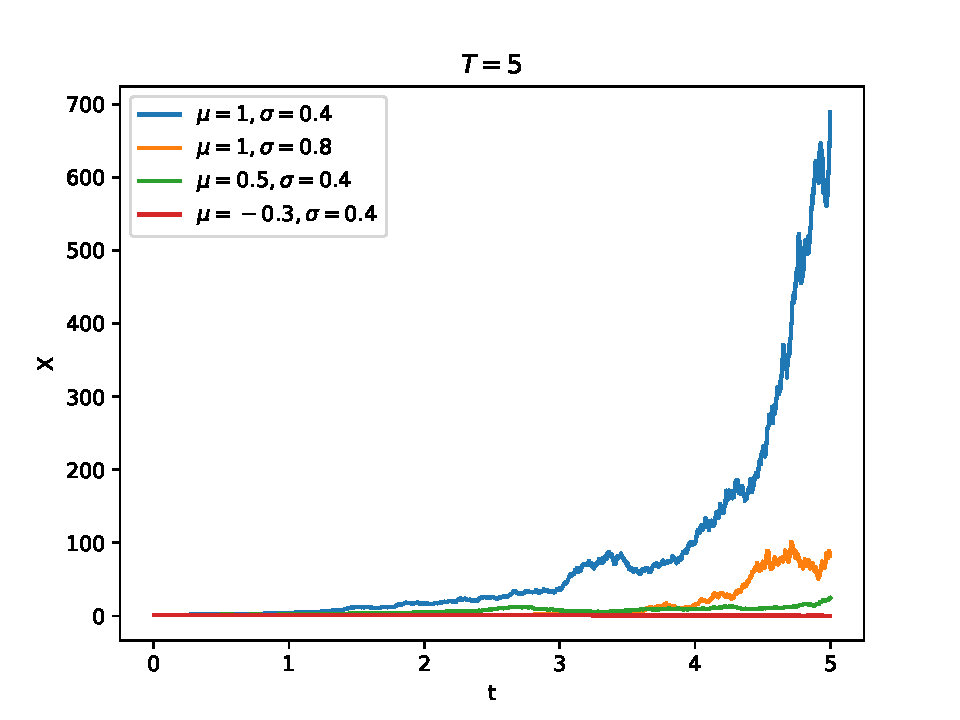
\includegraphics[width=0.47\textwidth]{T=5}
        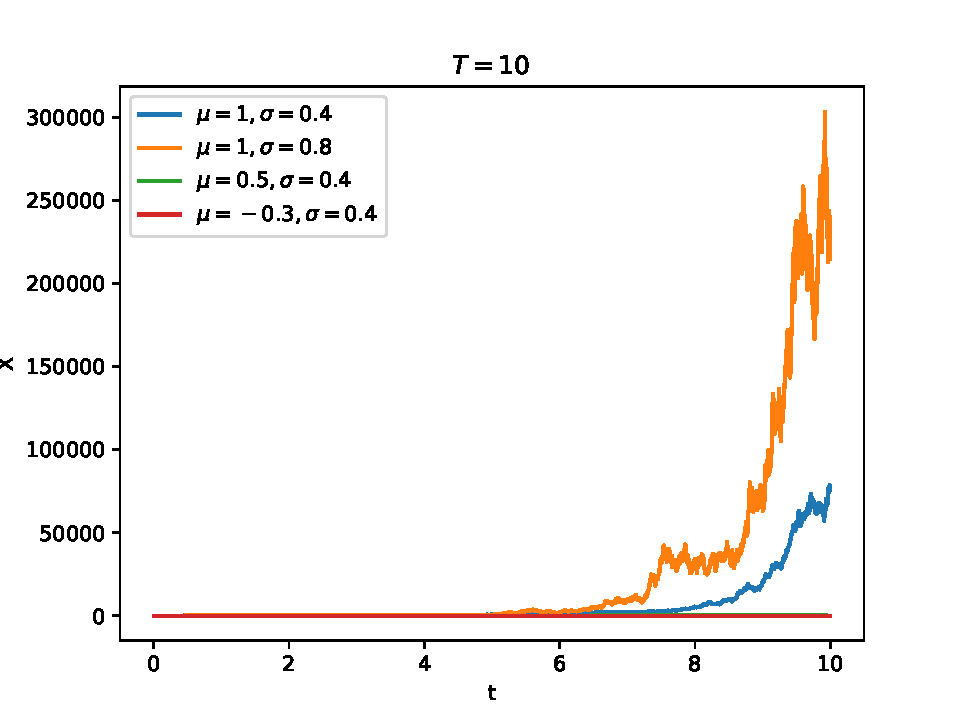
\includegraphics[width=0.47\textwidth]{T=10}
        \caption{Simulation of GBM}
        \label{fig:simulation}
    \end{figure*}

    \appendix
    \section{Python Code for Simulation}
    \begin{fullwidth}
    \lstinputlisting[language=Python]{simulator.py}
    \end{fullwidth}
\end{document}